%%%%%%%%%%%%%%%%%%%%%%%%%%%%%%%
% Author: Damodar Rajbhandari %
%%%%%%%%%%%%%%%%%%%%%%%%%%%%%%%

\documentclass[11pt]{beamer}
\usetheme{Warsaw}

\usepackage{graphicx}
\graphicspath{{pic/}{../pic/}}

\usepackage{hyperref}
\usepackage{anyfontsize}
\usepackage{tcolorbox}

\usepackage{xcolor}
\usepackage{colortbl}
\newcommand{\RowColor}{\rowcolor{gray!60}}

\usepackage{adjustbox}

\usepackage{tikzsymbols}

\usepackage{array}

\usepackage{amsmath}

\usepackage{listings}

\lstset
{
    language={[LaTeX]TeX},
    frame=single,
    framesep=\fboxsep,
    framerule=\fboxrule,
    rulecolor=\color{black},
    xleftmargin=\dimexpr\fboxsep+\fboxrule,
    xrightmargin=\dimexpr\fboxsep+\fboxrule,
    breaklines=true,
    basicstyle=\small\tt,
    keywordstyle=\color{blue}\sf,
    commentstyle=\color{purple!100},
    backgroundcolor=\color{gray!10},
    tabsize=2,
    columns=flexible,
}


\usenavigationsymbolstemplate{}

\author{Damodar Rajbhandari}
\title{A short introduction to \LaTeX \hspace{0.01cm} and it's importance}

\institute{{\color{blue} Out-reach Blogger at \\
 \href{www.physicslog.com}{www.physicslog.com}} \\
 \vspace{0.3cm} St. Xavier's College \\
 Kathmandu, Nepal}

\titlegraphic{\href{http://www.physicslog.com/}{
\includegraphics[width = 4cm, height = 0.5cm]{logo}}}
\date{2017}

%%%%%%%%%%%%%%%%%%%%%%%%%%%%%%%%%%%%%%%%%%%%%%%%%%%%%%%%%%%%%%%%%%%%%

\begin{document}


{\usebackgroundtemplate{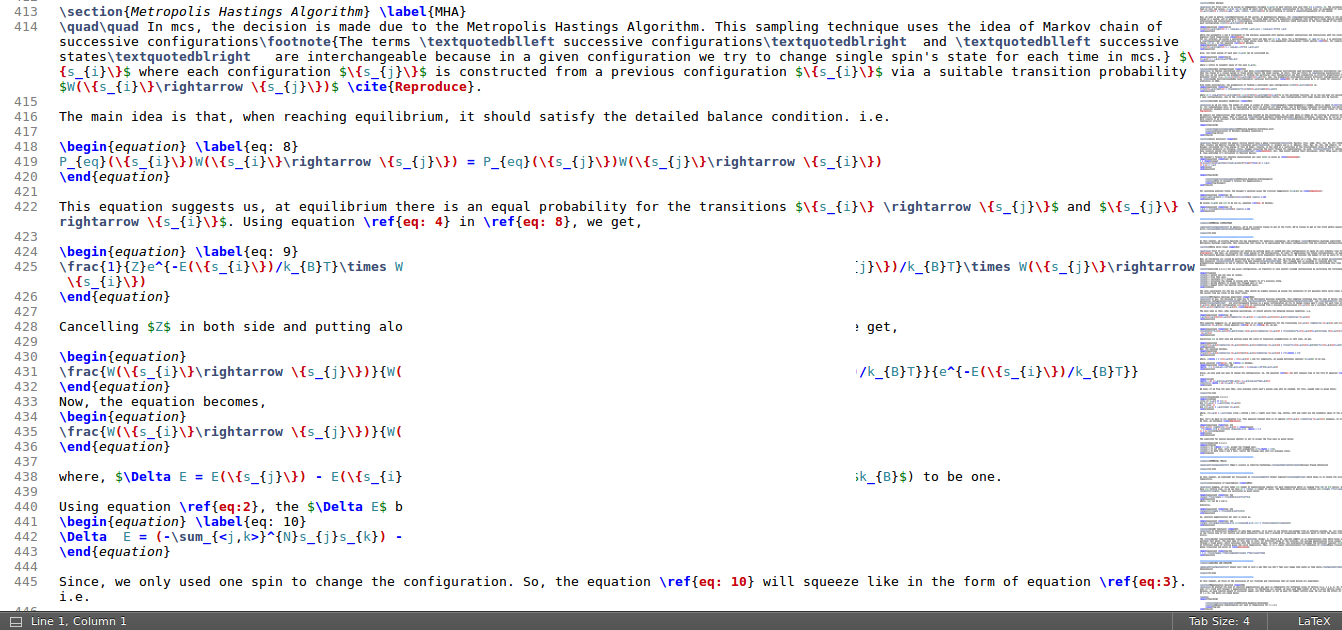
\includegraphics[width = 13.5cm, height = 9.5cm]{back}}
\frame{\titlepage}}

%%%%%%%%%%%%%%%%%%%%%%%%%%%%%%%%%%%%%%%%%%%%%%%%%%%%%%%%%%%%%%%%%%%%%%

\section[Table of contents]{}
\begin{frame}{Table of contents}
\tableofcontents
\end{frame}

%%%%%%%%%%%%%%%%%%%%%%%%%%%%%%%%%%%%%%%%%%%%%%%%%%%%%%%%%%%%%%%%%%%%%%%

\section{Info on \LaTeX}

%%%%%%%%%%%%%%%%%%%%%%%%%%%%%%%%%%%%%%%%%%%%%%%%%%%%%%%%%%%%%%%%%%%%%%
\subsection{Detail History}
\begin{frame}{Detail History}
\underline{\color{brown}History back to Typography (eg: \TeX) and Fonts}:\\
A well-respected computer scientist {\color{blue}\href{https://en.wikipedia.org/wiki/Donald_Knuth}{Donald Knuth}}:\\

\begin{itemize}

\item Published \textquotedblleft The Art of Computer Programming- Vol. 1\textquotedblright
\item Typeset in metal-typesetting system.

\item Publisher changed their printing technology into photo-typesetting.

\item In 30 March 1977, {\color{red}Disappointed} with the document quality of his book \textquotedblleft The Art of Programming- Vol. 2\textquotedblright. 


\pause

\vspace{0.2cm}
\underline{\color{brown}Issue}:

\item Letter wasn't position accurately.
\item Some words are more darker than others.

\pause

{\color{red} In short, No quality control over the document.}
 
\end{itemize}
\end{frame}

%%%%%%%%%%%%%%%%%%%%%%%%%%%%%%%%%%%%%%%%%%%%%%%%%%%%%%%%%%%%%%%

\begin{frame}{Detail History}
\underline{\color{brown} Inclined to think}:\

\begin{itemize}

\item During at Stanford, his community duty is to provide reading lists.

\item Same time 1977, he got a gallery proof of the book \textquotedblleft Artificial Intelligence\textquotedblright by {\color{blue}\href{https://en.wikipedia.org/wiki/Patrick_Winston}{Patrick Winston}}.  

\pause

\underline{\color{brown} Trigger point}:

\item Prepared using the machine that was completely digital.

\item It was typeset using pixels which encodes 0 and 1.

\pause

\underline{\color{brown} Clue}:

\item High quality printing is the matter of computer program. 

\item He saw it as in the form of computer problems.


\end{itemize}
\end{frame}


%%%%%%%%%%%%%%%%%%%%%%%%%%%%%%%%%%%%%%%%%%%%%%%%%%%


\begin{frame}{Detail History}

\underline{\color{brown} Beginning of \TeX}:
\begin{itemize}

\item Created a digital typesetting system i.e. \TeX

\item {\color{orange}Pronounce} as: /'t$\varepsilon$x/ tekh or {\color{violet}/'t$\varepsilon$k/ tek}.

\item Named from greek word $\tau \varepsilon \chi$ which means art as well as craft.
\item In 1978, Shared his software within the Permissive software licence.
\item Current stable version of \TeX\hspace{0.01cm} is 3.14159265 ($\pi$ with 8 decimals) which means, it's in the 9th version. 

\pause

\underline{\color{brown} Advantage}:
\item Gives extensive control of document layout.\\

\underline{\color{brown} Users using \TeX}:
\item \TeX\hspace{0.01cm} users were growing and they extended the macros.

\pause
\vspace{0.2cm}
\underline{\color{brown}Issue}:\\
\item Not easy to use ! 

\end{itemize}
\end{frame}

%%%%%%%%%%%%%%%%%%%%%%%%%%%%%%%%%%%%%%%%%%%%%%%%%%%%%%%%%%%%%%

\begin{frame}{Detail History}
\underline{\color{brown}Invention of \LaTeX}:

\begin{itemize}
\begin{tcolorbox}

\item Date back to 1985, {\color{blue}\href{https://en.wikipedia.org/wiki/Leslie_Lamport}{Leslie Lamport}} releases \LaTeX\hspace{0.01cm} to the modification of \TeX.

\item Aims to have a easy to use document preparation system.

\item \LaTeX\hspace{0.01cm} = \textquotedblleft {\color{purple}Lamport's \TeX}\textquotedblright

\item {\color{orange}Pronounce} as: /'la:t$\varepsilon$x/ LAH-tekh or /'leIt$\varepsilon$k/ LAY-tek or {\color{violet}/'la:t$\varepsilon$k/ LAH-tek}

\item Encloses with High Level Markup Language, which is syntactically distinguishable from the text.

\item File extension: {\color{blue}\textsf{*.tex}}

\end{tcolorbox}
\end{itemize}
\end{frame}

\subsubsection{Summary}
\begin{frame}{Summary}
\begin{tcolorbox}
\begin{center}

\bfseries \Large \TeX\hspace{0.01cm} is all about formatting, for designers\\
\& \\
\LaTeX\hspace{0.01cm} is all about content, for authors

\end{center}
\end{tcolorbox}
\end{frame}

\subsubsection{Motivation}
\begin{frame}{Motivation}
\begin{tcolorbox}
\begin{center}

\bfseries \Large \LaTeX\hspace{0.01cm} is easy to learn.

\end{center}
\end{tcolorbox}
\end{frame}

%%%%%%%%%%%%%%%%%%%%%%%%%%%%%%%%%%%%%%%%%%%%%%%%%%%%
\begin{frame}
\begin{center}
\Huge Any questions so far?
\end{center}
\end{frame}

%%%%%%%%%%%%%%%%%%%%%%%%%%%%%%%%%%%%%%%%%%%%%%%
\subsection{Why \LaTeX?}
\subsubsection{Battle between \textquotedblleft Word processor vs \LaTeX\textquotedblright}

\begin{frame}{Battle between \textquotedblleft Word processor vs \LaTeX\textquotedblright}

\begin{center}
{\large \underline{\textbf{Let's see, why some people started with word}}}
{\large \underline{\textbf{processor end up using \LaTeX \hspace{0.2cm}?}}}
\end{center}

\pause

\vspace{0.2cm}

\begin{tcolorbox}
\begin{center}
\textit{Sometimes the things that seems easier will put you in the hard situation!}
\end{center}
\end{tcolorbox}

\vspace{0.1cm}

\pause


\begin{tcolorbox}
\begin{center}
\drWalley[5][red] 
~
\pause
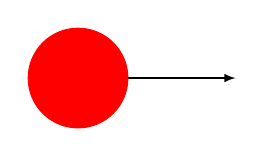
\begin{tikzpicture}[scale=2]

\draw[-latex] (0,0) coordinate (M) -- ++(1,0) [right];
\filldraw[red] (M) circle (9pt); 
\end{tikzpicture}
~
\pause
\dCooley[5][white]

\pause

{\Large{\textbf{Reason?}}}

\end{center}
\end{tcolorbox}




\end{frame}

\subsubsection{Reason}
\begin{frame}{Reason}

\begin{tabular}{|| c||c|c||}
\hline
\RowColor \textbf{Stuffs} & \textbf{Office Word, 1983} & \textbf{\LaTeX, 1985}  \\

\hline \hline \hline

\cellcolor{black} {\color{white} \raisebox{-1\height}{Logo}} & \raisebox{-.7\height}{
\includegraphics[width = 1cm, height = 1cm]{word}}  & \raisebox{-.7\height}{
\includegraphics[width = 1cm, height = 1cm]{latex}}\\
\hline \hline

\cellcolor{black} {\color{white} Handling Speed}
& Good for small docs & Good for large docs\\

\end{tabular}
\pause

\begin{tabular}{|| >{\centering}m{2.65cm}|| >{\centering}m{3.2cm}|  >{\centering}m{3.2cm} ||}
\hline \hline

{\cellcolor{black} {\color{white} Layout quality}}
& For general purpose it's okay!
& Good for professional purpose\\

\end{tabular}

\pause

\begin{tabular}{|| >{\centering}m{2.65cm}|| >{\centering}m{3.2cm}|  >{\centering}m{3.2cm} ||}

\hline \hline

{\cellcolor{black} {\color{white} Good handling Table \& Graphics}}\\
& For Small number\\
 & For large number\\

\end{tabular}

\begin{tabular}{ >{\centering}m{2.65cm} >{\centering}m{3.2cm}  >{\centering}m{3.52cm}}
\hline \hline 
& &
\end{tabular}


\end{frame}

\begin{frame}{Reason}

\begin{tabular}{|| >{\centering}m{2.65cm}|| >{\centering}m{3.2cm}|  >{\centering}m{3.2cm} ||}
\hline

{\cellcolor{black} {\color{white} Equations \& Symbols}}
& Time-consuming\\
& Easy\\
\end{tabular}
\pause

\begin{tabular}{|| >{\centering}m{2.65cm}|| >{\centering}m{3.2cm}|  >{\centering}m{3.2cm} ||}
\hline \hline

{\cellcolor{black} {\color{white} File Format}}
& Binary
& Plain-text
\end{tabular}

\pause

\begin{tabular}{|| >{\centering}m{2.65cm}|| >{\centering}m{3.2cm}|  >{\centering}m{3.2cm} ||}
\hline \hline

{\cellcolor{black} {\color{white} Version Control System supports }}
& No
& Yes 
\end{tabular}

\pause

\begin{tabular}{|| >{\centering}m{2.65cm}|| >{\centering}m{3.2cm}|  >{\centering}m{3.2cm} ||}
\hline \hline

{\cellcolor{black} {\color{white} Price}}
& Proprietary Commercial Software 
& Free Software

\end{tabular}


\begin{tabular}{ >{\centering}m{2.65cm} >{\centering}m{3.2cm}  >{\centering}m{3.52cm}}
\hline \hline 
& &
\end{tabular}

\end{frame}


\begin{frame}{In short:}
\begin{itemize}
\pause
\item High typographical quality of the document.
\pause
\item \LaTeX \hspace{0.1cm} allows users to clearly separate the content from the format of the document.
\pause
\item It gives user the opportunity to focus on \textquotedblleft what\textquotedblright the creative part of your work, rather than \textquotedblleft how\textquotedblright is it going to look when it get printed out.
\pause
\item It makes very simple to handle equations, figures, bibliography and index.
\pause
\item Programming kinda approach to putting the stuffs in the right place.
\end{itemize}

\end{frame}


\subsubsection{Lesson}

\begin{frame}{Lesson}

\begin{center}
\textbf{When to use word processor? \& 
When to use \LaTeX ?}

\pause

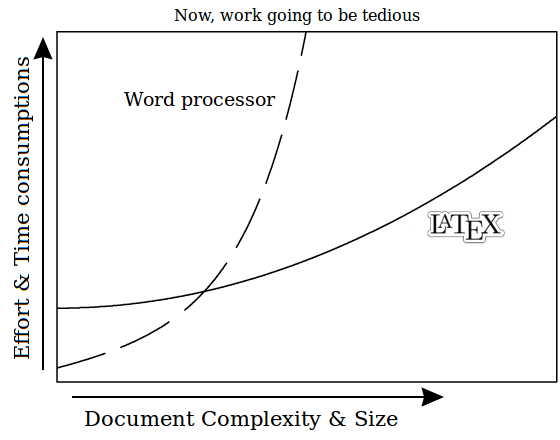
\includegraphics[width = 8cm, height = 6cm]{graph}
\end{center}
\end{frame}

\subsubsection{Motivation}

\begin{frame}{Motivation}

\begin{tcolorbox}
\begin{center}

\bfseries \Large \LaTeX\hspace{0.01cm} has more flexibility over your document and, powerful commands that makes your work easier and gives best results in least amount of time .

\end{center}
\end{tcolorbox}

\end{frame}

%%%%%%%%%%%%%%%%%%%%%%%%%%%%%%%%%%%%%%%%%%%%%%%%%%%%
\begin{frame}
\begin{center}
\Huge Any questions so far?
\end{center}
\end{frame}

%%%%%%%%%%%%%%%%%%%%%%%%%%%%%%%%%%%%%%%%%%%%%%%


\section{Tutorial}

\subsection{Setup}

\begin{frame}[fragile]
\frametitle{Setting up the \LaTeX\vspace{0.2cm} compiler and editor}

\begin{tcolorbox}
\textbf{For debian based Linux users:}\\
With internet connection, just type the following commands one after another within the existing terminal:
\begin{itemize}

\item \textsf{sudo apt-get install texlive-full}
\item \textsf{sudo apt-get install texmaker}
\end{itemize}
\end{tcolorbox}

\begin{tcolorbox}
\textbf{For Windows users:}
\begin{itemize}
\item \href{https://miktex.org/download}{Click Download} and install MiKTeX.
\item \href{http://www.xm1math.net/texmaker/}{Click Download} and install Texmaker.
\end{itemize}

\end{tcolorbox}
\end{frame}



\subsection{Basics}

\begin{frame}[fragile]
\frametitle{Understanding the \textsf{*.tex} document structure}


\begin{lstlisting}
\documentclass[Global parameter]{class.cls}
%[optional parameter]{calling design file}

%%%%%%%%%%%% Where we call necessary packages 
% Preamble %          &
%%%%%%%%%%%% redefine commands 
\usepackage{package_name}

\begin{document}
%%%%%%%%%%%%%%%%%%
% Your contents! % 
%%%%%%%%%%%%%%%%%%

\end{document}
\end{lstlisting}
\end{frame}

\begin{frame}{Understanding Document Type}
\begin{itemize}
\item article : For short documents and journal articles.\\ \hspace{1.28cm} Commonly used!
\item report : For longer documents and dissertations.
\item book : Useful to write books
\item letter : Useful to write letters
\item beamer : For presentations 
\end{itemize}

\end{frame}

\begin{frame}[fragile]
\frametitle{Knowing reserved characters}
The following symbol characters have a special meaning: 

\begin{center}
\begin{verbatim}
Character       Funtion,         How to print it?

#  Macro parameter,                     \#
$  Math mode,                           \$
%  Comment,                             \%
^  Superscript(in math mode),           \^{}  
&  Seperate column entries in tables,   \&
_  Subscript(in $ $),                   \_
{} Processing block,                    \{\}
~  Use it whenever you want to leave 
   a space which is unbreakable,        \~{}
\  Starting commands,                  $\backslash$
\end{verbatim}
\end{center}

\end{frame}

\begin{frame}[fragile]
\frametitle{Implementing our understanding using \textsf{article.cls} }

\begin{lstlisting}
\documentclass[a4paper, 12pt ]{article}

\usepackage[utf8]{inputenc} %Optional

\title{CDT 1+1 D without preferred foliation}
\author{Damodar Rajbhandari}
\date{2017} %Skip date using \date{}

\begin{document}

\begin{titlepage}
\maketitle
\end{titlepage}
% Now, Start filling your contents! 
\end{document}

\end{lstlisting}
\end{frame}


\begin{frame}[fragile]
\frametitle{Creating environment for specific use }

\begin{lstlisting}
...

\begin{document}
...
\begin{} %Fill environment in {}

%Created environment! 

\end{}

\end{document}

\end{lstlisting}
\end{frame}


\begin{frame}{Environments}

\begin{minipage}{0.3\linewidth}
\underline{Aligments:}
\begin{itemize}
\item center
\item flushleft
\item flushright

\end{itemize}
\end{minipage}
~
\pause
\begin{minipage}{0.63\linewidth}
\underline{Usefuls}
\begin{itemize}
\item tabular{\color{blue}*}
\item table{\color{blue}*}
\item matrix{\color{blue}*}
\item equation{\color{blue}*}
\item minipage{\color{blue} (small page within main page)}
\item verbatim{\color{blue} (for inserting codes)}
\item itemize{\color{blue}  (helps to create item)}
\item figure{\color{blue}*}

\vspace{0.2cm}
\item[*] {\color{blue} will be discussed it in more detail in the following section.}
\end{itemize}
\end{minipage}

\end{frame}


\begin{frame}[fragile]
\frametitle{Useful commands}
Here are the list of commands: 
\begin{verbatim}
\textbf{bold} \textit{italic} 
{\color{pick} text_here} %Changes the text color 

\vspace{scale} %vertical spacing
               %for eg: scale = 1cm 
\vspace*{scale} %for strictly follow this command! 

\hspace{scale} %for horizontal spacing
\hspace*{scale}  
\end{verbatim}
\end{frame}

\begin{frame}[fragile]
\frametitle{Useful commands}
 
\begin{verbatim}
\\ means line break 
\noindent means no indentation in starting paragraph
\underline{text_here} gives underline to the text.

\textquotedblleft  creates double-quote left
\textquotedblright creates double-quote right
 
\chapter{•}        creates chapter title
\section{•}        creates heading
\section*{•}       creates heading without labeling
\subsection{•}     creates sub-heading
\subsubsection{•}  creates sub-sub-heading

\end{verbatim}
\end{frame}

\begin{frame}[fragile]
\frametitle{Useful commands}
 
\begin{verbatim}

\tableofcontents   creates table of content
\listoffigures     list all the labelled figures.
\listoftables      list all the labelled tables.
\newpage           end up the page 
\pagenumbering{*}  can change numbering style like
                   arabic(1,2,...) to roman
                   (I, II,...) by putting it
                   instead of * 
                    
\end{verbatim}
{\color{blue}For maths commands, get it from the texmaker editor! }
\end{frame}

%%%%%%%%%%%%%%%%%%%%%%%%%%%%%%%%%%%%%%%%%%%%%%%%%%%%
\begin{frame}
\begin{center}
\Huge Any questions so far?
\end{center}
\end{frame}

%%%%%%%%%%%%%%%%%%%%%%%%%%%%%%%%%%%%%%%%%%%%%%%
\subsection{Building up some skills}

\begin{frame}[fragile]
\frametitle{Importing images*}

\begin{lstlisting}
...
\usepackage{graphicx}
\graphicspath{{your_folder/}{../your_folder/}}
%put all the images in the "your_folder" and this folder
%is outside from the folder of your LaTeX file.
\begin{document}
...
\includegraphics[width = ?cm, height = ?cm]{?image}}

%if you like: 
%[scale=?] %images in equal ratio in width & height
%[angle=?] %For eg: angle=45
\end{document}
\end{lstlisting}
{\color{red} *will not show in list of figures and cannot do cross-referencing!}
\end{frame}


\begin{frame}[fragile]
\frametitle{Position specifier}
\href{http://ctan.imsc.res.in/macros/latex/contrib/float/float.pdf}{Float*} {\color{blue}are used to contain contains things (i.e. tables and figures) that must be placed
inside a single page. }
\begin{verbatim}
Parameter               Position
   h           [Place the float* here, i.e.
               approximately at the same place
               where command is defined]
   t           [Position at the top of the page]
   b           [Position at the bottom of the page]
   !           [Override the internal parameters
               class file uses for determining 
               "good" float position]
   H           [Precisely place here, need float
               package, equivalent to h!]
\end{verbatim}

\end{frame}


\begin{frame}[fragile]
\frametitle{Exploration on inserting images}

\begin{lstlisting}
...
\begin{document}
\listoffigures
...
\begin{figure}[position specifier]

\includegraphics[width = ?cm, height = ?cm]{?image}}
\caption{?Will be shown in list of figures!}
\label{fig:?for cross-referencing}

\end{figure}
...\ref{fig:?for cross-referencing}
\end{document}
\end{lstlisting}
\end{frame}

\begin{frame}{Some suggestions on graphics}
\begin{itemize}
\item Use vector images(for eg. \textsf{*.ps} and \textsf{*.pdf}) rather than raster images(for eg. \textsf{*.png}) so that, the resolution is in good quality.\\
\pause
\vspace{0.2cm}

{\small \bfseries \underline{Vector images} are created in drawing programs. This program uses points connected with curves or straight lines, like connect-the-dots. The advantage of using this images is that it is resolution independent.\\
But, \underline{Raster or bitmapped images} uses pixels to define images.}
\pause
\item Do not use spaces while naming the images. 
\pause
\item Choose file names that is specific and descriptive.
\pause
\item Put all the images in one folder.

\end{itemize}
\end{frame}


%%%%%%%%%%%%%%%%%%%%%%%%%%%%%%%%%%%%%%%%%%%%%%%%%%%%
\begin{frame}
\begin{center}
\Huge Any questions so far?
\end{center}
\end{frame}

%%%%%%%%%%%%%%%%%%%%%%%%%%%%%%%%%%%%%%%%%%%%%%%

\begin{frame}[fragile]
\frametitle{Understanding tables}
\begin{verbatim}
Parameter          Meaning
l            left-justified column
c            centered column
r            right-justified column
|            vertical line
||           double vertical line
&            column separator
\\           start new row
\hline       horizontal line
\end{verbatim}
\end{frame}


\begin{frame}[fragile]
\frametitle{Inserting table*}
\begin{minipage}{0.5\linewidth}


\begin{lstlisting}
...
\begin{document}
...
\begin{tabular}{||c|c||}
\hline
Parameter & Meaning\\
\hline
l & left-justified\\
c & centered column\\
\hline 
\end{tabular}

\end{document}
\end{lstlisting}
\end{minipage}
~
\begin{minipage}{0.45\linewidth}
\textbf{Output:}\\
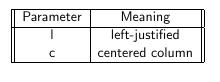
\includegraphics[scale=0.6]{table}
\end{minipage}
{\color{red} *will not show in list of tables and cannot do cross-referencing!}
\end{frame}


\begin{frame}[fragile]
\frametitle{Exploration on inserting tables}

\begin{lstlisting}
\begin{document}
\listoftables 
\begin{table}[position specifier]
\begin{tabular}{||c|c||}
\hline
Parameter & Meaning\\
\hline
l & left-justified\\ %Not forgot to add \\ at the end
c & centered column\\ 
\hline 
\end{tabular}
\caption{?Will be shown in list of tables!}
\label{table:?for cross-referencing}
\end{table}
... \ref{table:?for cross-referencing}

\end{lstlisting}
\end{frame}




%%%%%%%%%%%%%%%%%%%%%%%%%%%%%%%%%%%%%%%%%%%%%%%%%%%%
\begin{frame}
\begin{center}
\Huge Any questions so far?
\end{center}
\end{frame}

%%%%%%%%%%%%%%%%%%%%%%%%%%%%%%%%%%%%%%%%%%%%%%%



\begin{frame}[fragile]
\frametitle{Creating Matrix}

\begin{minipage}{0.4\linewidth}
\begin{lstlisting}
...
\usepackage{amsmath}
\begin{document}
...
$\begin{matrix} 
a & b \\
c & d 
\end{matrix}$
...
$
\begin{pmatrix} 
a & b \\
c & d 
\end{pmatrix}$
...

\end{lstlisting}
\end{minipage}
~
\begin{minipage}{0.4\linewidth}

\begin{lstlisting}
$\begin{bmatrix} 
a & b \\
c & d 
\end{bmatrix}
\quad
\begin{vmatrix} 
a & b \\
c & d 
\end{vmatrix}
\quad
\begin{Vmatrix} 
a & b \\
c & d 
\end{Vmatrix}
$ ...

\end{lstlisting}
\end{minipage}

\end{frame}



\begin{frame}{contd.}
\textbf{Output:}\\
\vspace*{0.2cm}
 
$\begin{matrix} 
\hspace*{0.3cm} a & b \\
\hspace*{0.3cm} c & d 
\end{matrix}
\linebreak 
$
\vspace*{0.2cm}

$\begin{pmatrix} 
a & b \\
c & d 
\end{pmatrix}
\linebreak
$

\vspace*{0.2cm}

$
\begin{bmatrix} 
a & b \\
c & d 
\end{bmatrix}
\quad
\begin{vmatrix} 
a & b \\
c & d 
\end{vmatrix}
\quad
\begin{Vmatrix} 
a & b \\
c & d 
\end{Vmatrix}
$

\end{frame}

%%%%%%%%%%%%%%%%%%%%%%%%%%%%%%%%%%%%%%%%%%%%%%%%%%%%
\begin{frame}
\begin{center}
\Huge Any questions so far?
\end{center}
\end{frame}

%%%%%%%%%%%%%%%%%%%%%%%%%%%%%%%%%%%%%%%%%%%%%%%



\begin{frame}[fragile]
\frametitle{Inserting equation}

\begin{lstlisting}
...
\usepackage{amsmath} %important package

\begin{document}
...
\begin{equation} \label{eq:eg}

S = \frac{1}{8\pi G}\int d^{4}\times\sqrt{\det(g_{\mu\nu})}\left(\Lambda-\frac{1}{2}R\right)

\end{equation}
Equation \ref{eq:eg} is known as Einstein-Hilbert Action with no matter coupling. 
% To do cross-referencing, we have used \ref{} command.
...

\end{lstlisting}
\end{frame}

\begin{frame}{contd.}
\textbf{Output:}
\begin{equation} \label{eq:eg}
S = \frac{1}{8\pi G}\int d^{4}x\sqrt{\det(g_{\mu\nu})}\left(\Lambda-\frac{1}{2}R\right)
\end{equation}
 
Equation \ref{eq:eg} is known as Einstein-Hilbert Action with no matter coupling.
\end{frame}


\begin{frame}[fragile]
\frametitle{Exploration on inserting equation}
\begin{lstlisting}
...
\usepackage{amsmath} %mandatory package
\begin{document}
...
\begin{align}

S &= \frac{1}{8\pi G}\int d^{4}\times\sqrt{\det(g_{\mu\nu})}\left(\Lambda-\frac{1}{2}R\right)  \\   
%Useful character is &
&\Leftrightarrow \frac{1}{8\pi G}\sum_{j\epsilon T}\left( \Lambda\frac{\sqrt{5}}{4}a^{2}n_{j}(T)-\delta_{j}\right) 

\end{align} 
...
\end{document}
\end{lstlisting}
\end{frame}



\begin{frame}{contd.}
\textbf{Output:}
\begin{align}
S &= \frac{1}{8\pi G}\int d^{4}x\sqrt{\det(g_{\mu\nu})}\left(\Lambda-\frac{1}{2}R\right)  \\   
&\Leftrightarrow \frac{1}{8\pi G}\sum_{j\epsilon T}\left( \Lambda\frac{\sqrt{5}}{4}a^{2}n_{j}(T)-\delta_{j}\right) 
\end{align}  
\end{frame}


\begin{frame}[fragile]
\frametitle{contd.}
\begin{lstlisting}
...
\begin{align}
S &= \frac{1}{8\pi G}\int d^{4}\times\sqrt{\det(g_{\mu\nu})}\left(\Lambda-\frac{1}{2}R\right)  \nonumber \\   
%Useful command: \nonumber
&\Leftrightarrow \frac{1}{8\pi G}\sum_{j\epsilon T}\left( \Lambda\frac{\sqrt{5}}{4}a^{2}n_{j}(T)-\delta_{j}\right) \label{eg2}
%Useful command: \label{}
\end{align}
Thus, we have converted Einstein-Hilbert action in smooth manifold with no matter coupling into Regge action in discretized triangulated manifold (i.e. equation \ref{eg2}).
...
\end{lstlisting}
\end{frame}


\begin{frame}{contd.}
\textbf{Output:}
\begin{align}
S &= \frac{1}{8\pi G}\int d^{4}x\sqrt{\det(g_{\mu\nu})}\left(\Lambda-\frac{1}{2}R\right)  \nonumber \\   
&\Leftrightarrow \frac{1}{8\pi G}\sum_{j\epsilon T}\left( \Lambda\frac{\sqrt{5}}{4}a^{2}n_{j}(T)-\delta_{j}\right) \label{eg2}
\end{align}
Thus, we have converted Einstein-Hilbert action in smooth manifold with no matter coupling into Regge action in discretized triangulated manifold (i.e. equation \ref{eg2}).  
\end{frame}



%%%%%%%%%%%%%%%%%%%%%%%%%%%%%%%%%%%%%%%%%%%%%%%%%%%%
\begin{frame}
\begin{center}
\Huge Any questions so far?
\end{center}
\end{frame}

%%%%%%%%%%%%%%%%%%%%%%%%%%%%%%%%%%%%%%%%%%%%%%%



\begin{frame}[fragile]
\frametitle{Bibliography: Bibtex}
We'll create bibliography using Bibtex rather than thebibliography environment({\color{brown}\href{https://www.sharelatex.com/learn/Bibliography_management_with_bibtex}{if you like, click how!}}). Here are the following steps:
\begin{itemize}
\item Create a new file in the texmaker.
\item Click {\color{blue}Bibliography} menu Then, {\color{blue}Bibtex}.
\item Choose which type of document you want to cite. For eg: \textquotedblleft Article in Journal\textquotedblright.
\item Then, you will see like:

\end{itemize}

\end{frame}


\begin{frame}[fragile]
\frametitle{contd.}
\begin{lstlisting}
@Article{*, % this line * means label for citation.
author = {*},
title = {*},
journal = {*},
year = {*},
OPTkey = {*},    % OPT means optional 
OPTvolume = {*}, %if you want to put volume then,
                 %remove OPT and make it volume = {*}
OPTnumber = {*}, %if you donot need these just remove it.
OPTpages = {*},
OPTmonth = {*},  %never forget "comma"
OPTnote = {*},
OPTannote = {*}  
}
\end{lstlisting}
\end{frame}

\begin{frame}[fragile]
\frametitle{contd.}

\begin{itemize}
\item Fill the information as:
\end{itemize}
\begin{lstlisting}
@Article{cdt, 
author = {Joshua H. Cooperman and Jonah M. Miller},
         %if there are more than two authors then,
         %add by putting "and" one after another.       
title = {A first look at transition amplitude in (2+1)-dimensional causal dynamical triangulation},
journal= {Classical and Quantum Gravity},
volume= {31},
pages= {035012},
year= {2014}
}
\end{lstlisting}
{\color{red}Removed which are not used!}
\end{frame}

\begin{frame}[fragile]
\frametitle{contd.}

\begin{itemize}
\item Save it as {\color{blue}?bibfile.bib} and should be within the same folder of your document's tex file.
\end{itemize}
\begin{lstlisting}
\begin{document}
...\cite{cdt} %Creates citation! 
...\citep{cdt} %creates citation with parenthesis!
...\citep{cdt,cdt} %creates multiple citation using comma

%if you want to put footnote then, use this command:
% \footnote{your_text_here!}

\bibliographystyle{apa}
%choose another instead of apa, if you like!
\bibliography{?bibfile}
\end{document}
\end{lstlisting}
\end{frame}

\begin{frame}[fragile]
\frametitle{contd.}

\begin{itemize}
\item Now, compile it by clicking:
\item[1.] PDFLaTeX
\item[2.] BibTeX
\item[3.] PDFLaTeX
\item[4.] PDFLaTeX {\color{blue}(this one is for sure!)}
\item Check the pdf.
\end{itemize}
\end{frame}


%%%%%%%%%%%%%%%%%%%%%%%%%%%%%%%%%%%%%%%%%%%%%%%%%%%%
\begin{frame}
\begin{center}
\Huge Any questions so far?
\end{center}
\end{frame}

%%%%%%%%%%%%%%%%%%%%%%%%%%%%%%%%%%%%%%%%%%%%%%%






%%%%%%%%%%%%%%%%%%%%%%%%%%%%%%%%%%%%%%%%%%%%%%%%%%%
\subsection{Extra Packages}

\begin{frame}{How to install extra packages}

\textbf{\underline{Error}}: \textquotedblleft class file\textquotedblright or \textquotedblleft package file\textquotedblright not found.\\

\textbf{\underline{Means}}: Package needs to be installed.\\
\textbf{\underline{Steps}}:\\
\vspace{0.2cm}
\textbf{[1] \underline{For linux users*}}:
\begin{itemize}
\item First, you need to have \textsf{texlive-full} installed.
\item Know which file is missing by seeing in Message/Log of Texmaker.
\item Open the terminal.
\item Type: \textsf{cd /usr/share/texlive/texmf-dist/tex/latex}
\item Make a directory to make your files organize as by typing: \textsf{sudo mkdir ?package\_dir}
\item Download \& extract the package from \href{https://www.ctan.org/}{Comprehensive \TeX\hspace{0.2cm} Archive Network(CTAN)} or any resources.

\end{itemize} 
\end{frame}

\begin{frame}{contd.}
\begin{itemize}

\item Copy the file, by typing:\\{\footnotesize \textsf{sudo cp /home/?username/Downloads/?package/?.sty  ./?package\_dir}}\\
{\color{red}Don't copy \textsf{*.bst}. The bst file will go in the /bibtex/bst directory. And, it should be known that other files(i.e. \textsf{*.tex, *.pdf, *.dvi}) are likely documentation for the package.} 
\item Update the filename database using the texhash command by typing:\textsf{ sudo texhash}\\
{\color{blue}Messages about texhash updating, then done.}

\vspace{0.4cm}
\pause
{\color{purple}\underline{Motivation}: I just wanted to teach you some commands in linux terminal. \dLaughey}

\end{itemize}
\end{frame}

\begin{frame}{contd.}
\textbf{[*] \underline{Simplest way}}:
\begin{itemize}
\item Know which package is missing from the Message/Log of Texmaker.
\item Download the required package and extract it.
\item Put the \textsf{?.sty} file inside the folder where your document source code \textsf{?.tex} is in! 
\item Click Quick build in the texmaker!
\item It will automatically install that package in the texlive package directory.

{\color{blue}I haven't yet got issue\footnote{If you find issue then, shot me an email at \texttt{dphysicslog@gmail.com} and we will together solve that problem.} while following this step! \dSmiley}
\end{itemize}
\end{frame}


\begin{frame}{contd.}
\textbf{[2] \underline{For Windows users}}:
\begin{itemize}

\item Click \textit{Windows key} and search \textit{miktex package manager}. 
\item Open it and search the package you want! \\
{\color{red} Need internet connection!}
\item Install it! \\
\pause
{\color{blue}But, if you have package downloaded then, follow the below steps:}\\
\pause
\item Copy the package file and paste to the path \textsf{Local disk C $\rightarrow$ Program Files $\rightarrow$ MiKTeX 2.9 $\rightarrow$ tex $\rightarrow$ latex $\rightarrow$ ?package\_dir (create a folder)$\rightarrow$ paste it here! }
\item Then, click \textit{Windows key} and search \textit{miktex settings(Admin)}.
\item Open it and click \textit{Refresh FNDB\footnote{FNDB means File Name Database}} then, click \textit{OK}.\\
 
\end{itemize}
\end{frame}

%%%%%%%%%%%%%%%%%%%%%%%%%%%%%%%%%%%%%%%%%%%%%%%%%%%%
\begin{frame}
\begin{center}
\Huge Any questions so far?
\end{center}
\end{frame}

%%%%%%%%%%%%%%%%%%%%%%%%%%%%%%%%%%%%%%%%%%%%%%%

\begin{frame}{List of useful packages*}
\begin{itemize}
\item comment {\color{blue}(helps to create multiline comment)*}
\item float    {\color{blue}(puts graphics in desired position)*}
\item imakeidx {\color{blue}(Creates index)*}
\item nomencl  {\color{blue}(Creates list of abbreviations)*}
\item geometry {\color{blue}(helps to modify the layout)}
\item hyperref {\color{blue}(use to create hyperlink)}
\item fancyhdr {\color{blue}(use to design header and footer)}
\item mathptmx {\color{blue}(for \href{http://ctan.org/pkg/mathptmx}{\color{brown}Times New Roman})}

\vspace{0.2cm}
\item[*] {\color{blue} will be discussed it in more detail in the following section.}

\end{itemize}
\end{frame}

\begin{frame}[fragile]
\frametitle{Package: \href{http://tug.ctan.org/macros/latex/contrib/comment/comment.sty}{comment} }

\begin{lstlisting}
...
\usepackage{comment}
\begin{document}
...
\begin{comment}

Fill your comments! 
For multi-line comments.

\end{comment}
\end{document}

\end{lstlisting}
\end{frame}


\begin{frame}[fragile]
\frametitle{Package: \href{http://www.ics.uci.edu/~rickl/cs-175/format/tex/float.sty}{float}}

\begin{lstlisting}
...
\begin{document}
\listoffigures
...
\begin{figure}[H]

\includegraphics[width = ?cm, height = ?cm]{?image}}
\caption{?Will be shown in list of figures!}
\label{fig:?for cross-referencing}

\end{figure}
...
\ref{fig:?for cross-referencing}
\end{document}
\end{lstlisting}
{\color{blue} \href{https://en.wikibooks.org/wiki/LaTeX/Floats,_Figures_and_Captions}{See} \href{http://tug.ctan.org/macros/latex/contrib/wrapfig/wrapfig.sty}{wrapfig} package for better handling the images.}
\end{frame}

\begin{frame}[fragile]
\frametitle{Package: imakeidx}

\begin{lstlisting}
...
\usepackage{imakeidx}
\makeindex
\begin{document}

...\index{Quantum Gravity} Quantum Gravity...

\appendix
... %Creating any chapter refers to appendices 

\bibliographystyle{stylename}
\bibliography{bibfile}

\printindex 
\end{document}

\end{lstlisting}
\end{frame}

\begin{frame}[fragile]
\frametitle{Package: nomencl}

\begin{lstlisting}
\usepackage{nomencl}
\makenomenclature
\renewcommand{\nomname}{List of Abbrevations}
\begin{document}
...
\printnomenclature
%put the above command where you want to see list of abbrevations.
\newpage
...
CDT \nomenclature{CDT}{Causal Dynamical Triangulation} is one of the candidate of \nomenclature{QG}{Quantum Gravity} Quantum Gravity.
...
\end{document}

\end{lstlisting}
\end{frame}


\begin{frame}{Understanding minor errors like:}
\begin{itemize}
\item vbox message 
\item hbox message
\item Missing \$ inserted.
\item ?package.file\_extension (for eg: damodar.sty) file not found.

\end{itemize}
\end{frame}

\section{Acknowledgements}
\begin{frame}{References}
Here are the list of resources where i learned alot of things on \LaTeX.
\begin{itemize}
\item \href{https://www.sharelatex.com/learn/}{ShareLaTeX}
\item \href{https://tex.stackexchange.com/}{\TeX\hspace{0.1cm} Stack Exchange}
\item \href{https://www.overleaf.com/latex/templates}{Overleaf}
\item \href{https://www.overleaf.com/latex/templates}{Wikibooks}

\end{itemize}

\end{frame}

\begin{frame}{Special thanks}
\begin{center}
\bfseries
I would to express my deep gratitude to my on-going cdt's supervisor \href{http://www.thephysicsmill.com/}{Jonah Maxwell Miller} for always inspiring me to do interesting things. \\

\end{center} 
\end{frame}

\begin{frame}{Special page}
\begin{center}
{\Large \bfseries Dedication\\ To\\ My Late Father}\\
who is in heaven
\end{center}
\end{frame}

\begin{frame}{Special page}
\begin{center}
\bfseries
On a personal note, I would like to thank to my parents especially to my Uncle and Aunt, whose continued love, encouragement, best wishes, support, and belief in my abilities have made it possible for me to go from very mediocre student to a good standing student.\\
\vspace{0.1cm}
Foremost, thanks to Dipika and Swastika for being a part of my life. Without their emotional support upto now, i might never succeed to stand at this position. 
\end{center}
\end{frame}

\begin{frame}{Final words!!!}

\begin{center}
\textbf{{\large \underline{Assignment}}\\
Keep this presentation file\footnote{This presentation file is prepared using beamer \LaTeX\hspace{0.1cm} class. Find a copy of source code at \url{https://github.com/damicristi/latex} and presentation file at \url{https://physicslog.com/about-author}} as a guide!\\
Create an empty \LaTeX\hspace{0.1cm} document and implement all the stuffs that you have learned today!}\\
\vspace{1cm}

{\Large \dSmiley THANK YOU FOR YOUR KIND PATIENCE \dSmiley}
\end{center}
\end{frame}


%HURRAY! I FINALLY DID IT!
\end{document}

